\section{Mean free path}
\section{Slip length}
\section{Mass continuity equation}

\section{Darcy's law for gases}
\label{sec:darcy_gas}
Darcy's law tells us what volumetric flow rate $Q$ one would expect from a liquid with viscosity $\mu$ through a material with permeability $k$ of length $L$ and volume $V$ when we apply a pressure difference $\Delta P$, see figure \ref{fig:darcys_law}. 
\begin{figure}[h]
\begin{center}
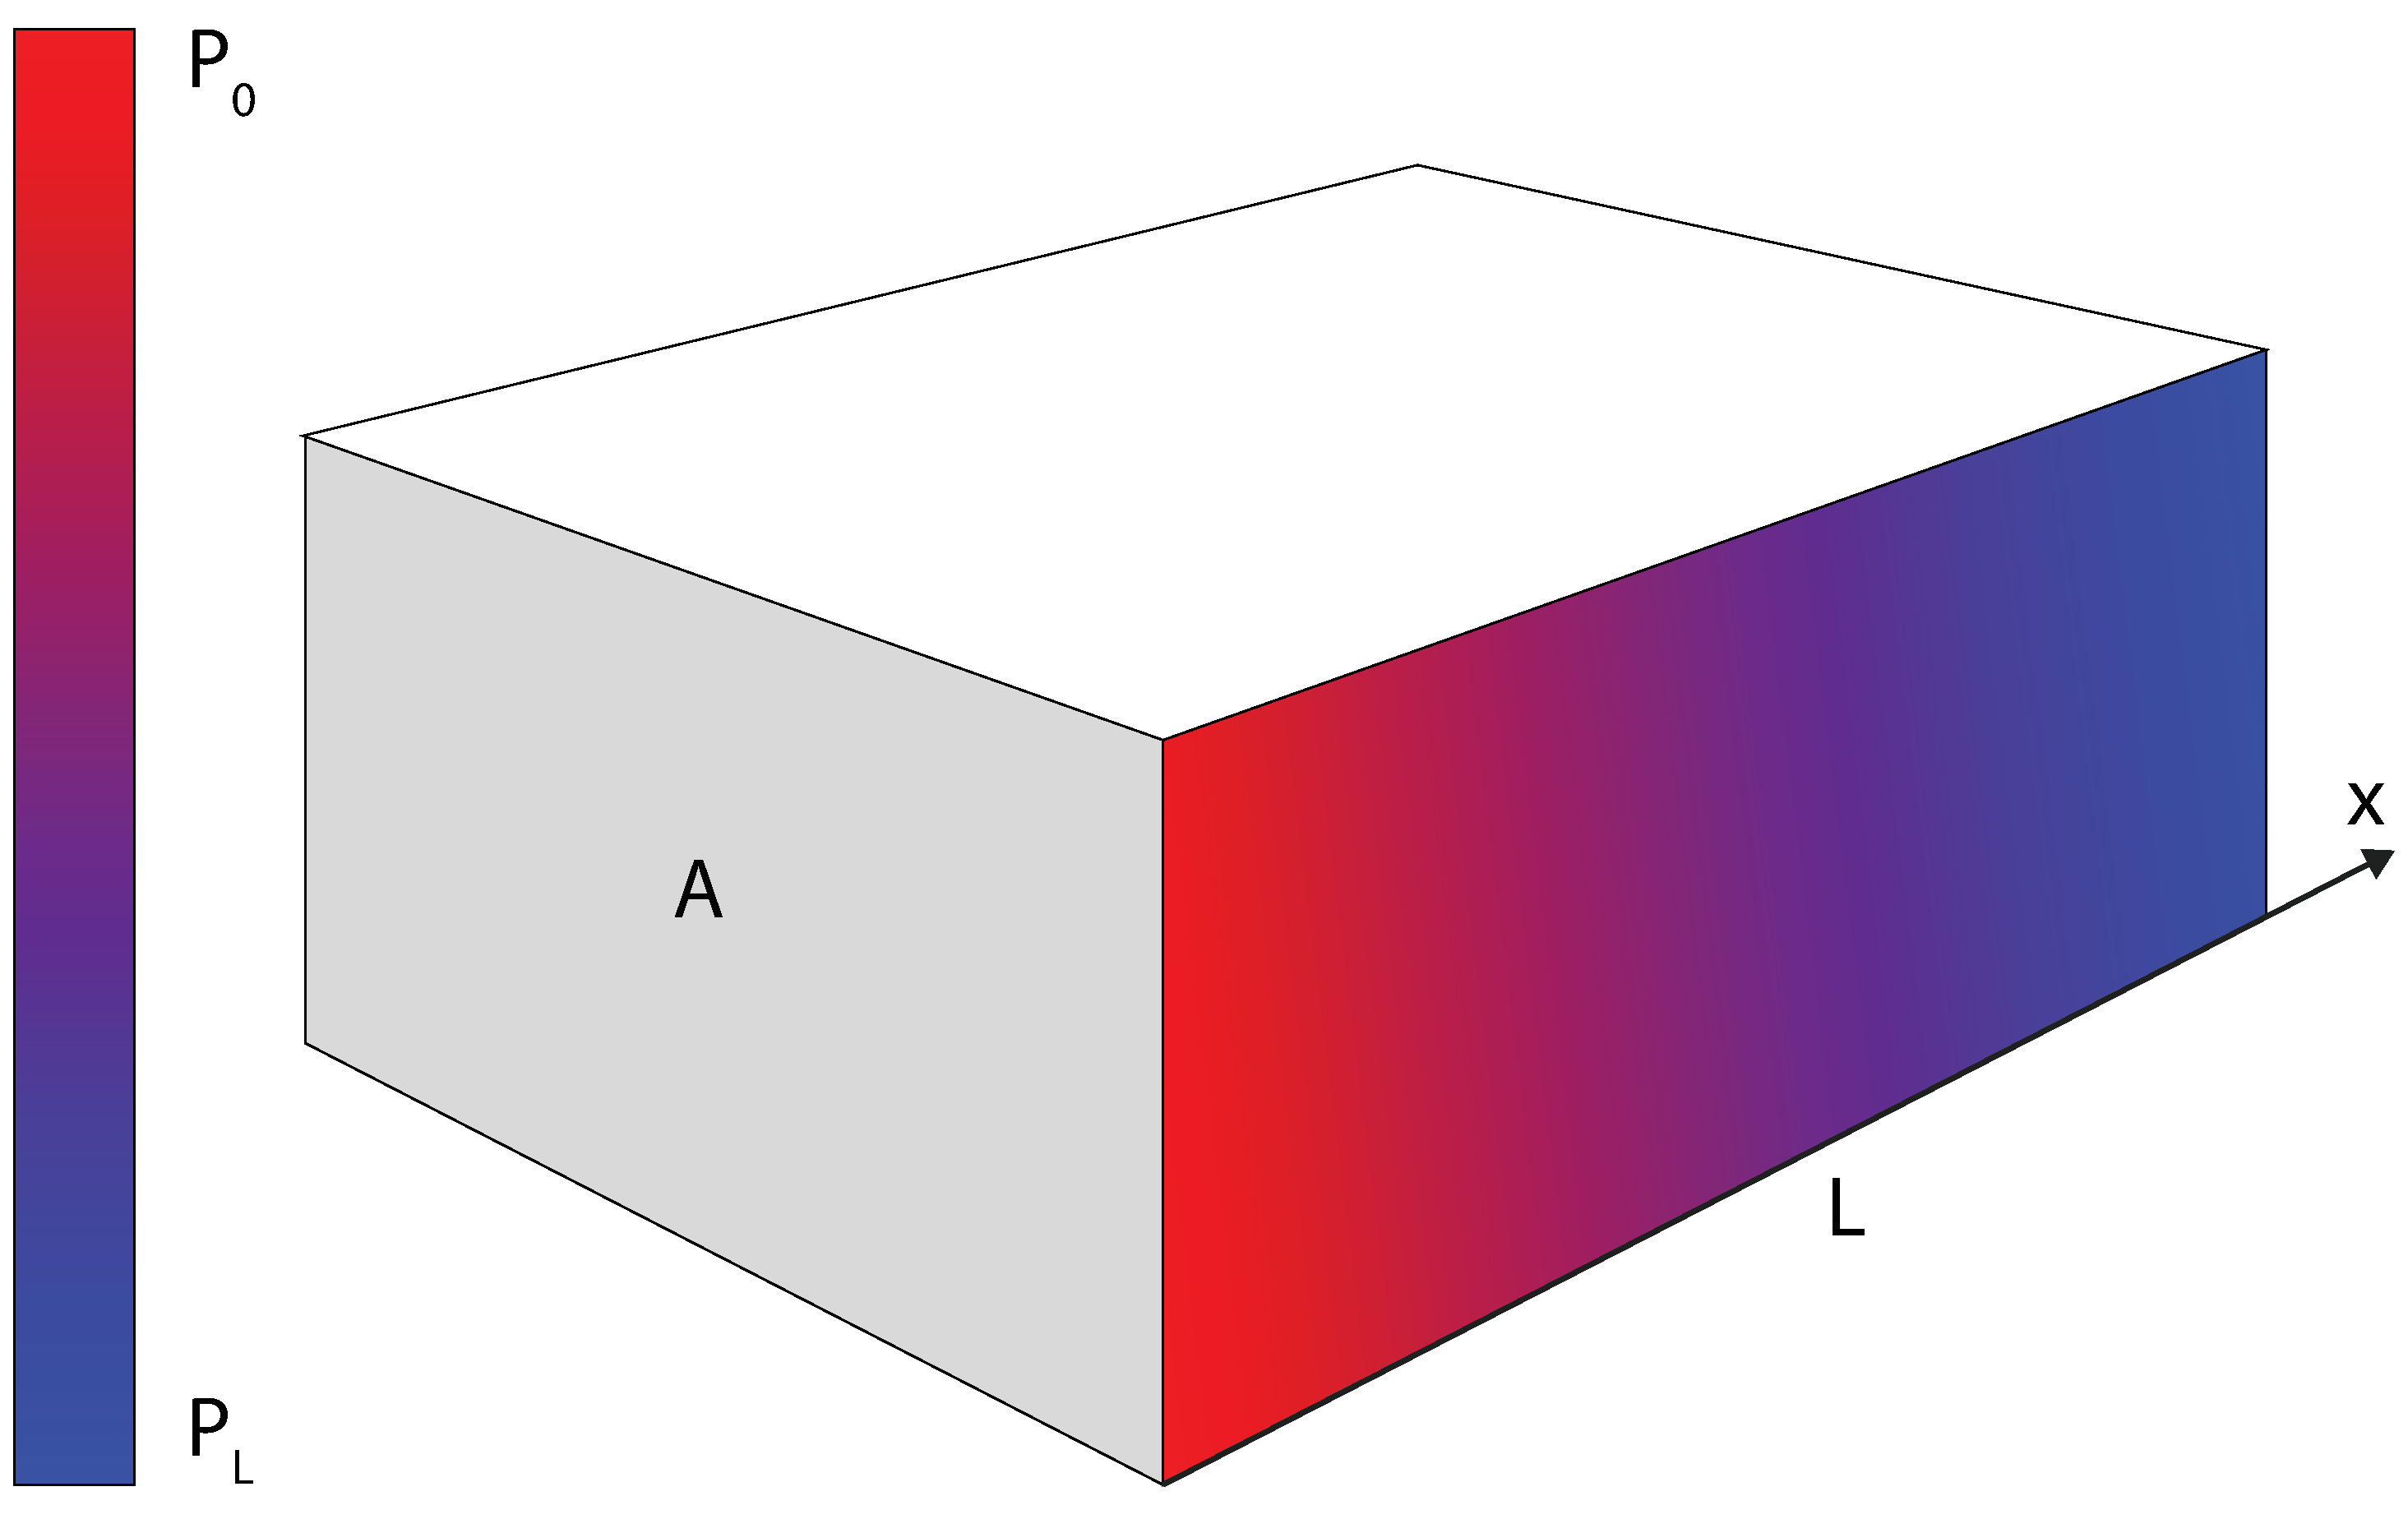
\includegraphics[width=\textwidth, trim=0cm 0cm 0cm 0cm, clip]{kinetic_theory/figures/darcy.eps}
\label{fig:darcys_law}
\end{center}
\caption{A box with volume $V=LA$ with fixed pressure values at $x=0$ and $x=L$.}
\end{figure}
Since we usually operate with flow in one direction, we will only look at the one dimensional version of Darcy's equation which is given as
\begin{align}
\label{eq:darcy_1}
	Q = A{k\over \mu}{\Delta P\over L},
\end{align}
where $A$ is the cross sectional area; the area of the plane orthogonal on the flow direction. By letting $L\rightarrow 0$, we get the differential form of Darcy's law
\begin{align}
\label{eq:darcy_2}
	Q = -A{k\over \mu}{dP\over dx},
\end{align}
where we picked up a minus sign because the fluid flows from high pressure to low pressure. One of the assumptions in the derivation of Darcy's law is that the liquid is incompressible.\cite{darcy_derivation} This is a bad approximation for gases, so we need a similar equation that allows non-constant densities. We rewrite Darcy's law by instead using the volumetric flux (or Darcy velocity) $u=Q/A$
\begin{align}
	\label{eq:darcy_3}
	u = -{k\over \mu}{dP\over dx}.
\end{align}
We then assume that the gas satisfies the ideal gas equation of state
\begin{align}
	P = \rho_n kT,
\end{align}
where $P$ is the pressure, $k_B$ is Boltzmann's constant and $T$ is the temperature. The mass continuity equation states that
\begin{align}
	\dpart{(\phi \rho_m)}{t} + \dpart{(u\rho_m)}{x} = 0,
\end{align}
which at a steady state is reduced to
\begin{align}
	\dpart{(\rho_m u)}{x} = 0,
\end{align}
which in turn gives that $\rho_m u$ is a constant and can be written as
\begin{align}
	\rho_m u = {Pm\over k_BT} c,
\end{align}
where we have applied the ideal gas law. We can solve for the Darcy velocity $u$ and insert this into equation \eqref{eq:darcy_3}
\begin{align}
	{ck_BT\over P m} &= -{k\over \mu}{dP\over dx}\\
	{ck_BT\over m}dx &= -{k\over \mu}pdP,
\end{align}
and integrate 
\begin{align}
\nonumber
	{ck_BT\over m}\int_0^L dx &= -{k\over \mu}\int_{P_0}^{P_L} pdP\\
\nonumber
	{ck_BT\over m}L &= -{k\over 2\mu}\left(P_L^2 - P_0^2\right)\\
\nonumber
	u &= {k\over 2\mu}{\left(P_0^2 - P_L^2\right)\over PL}\\
\label{eq:darcy_gas}
	Q &= A{k\over 2\mu}{\left(P_0^2 - P_L^2\right)\over PL}
\end{align}
where $u$ and $P$ is measured at the same point $x$. 
